\chapter{Análisis de faltas a tierra en AT}
\section{Componentes simétricas}
Se divide un sistema trifásico en 3 componentes, directa, inversa y homopolar.
Vector unitario a:
\begin{equation}
	a=1\angle\ang{120}
\end{equation}
\begin{itemize}
	\item SD
	\begin{itemize}
		\item $U_{a1}=U\angle \delta=U_{a1}$ 
		\item $U_{b1}=U\angle \delta -\ang{120}=a^2U_{a1}$
		\item $U_{c1}=U\angle \delta -\ang{240}=aU_{a1}$
	\end{itemize}
	\item SI
	\begin{itemize}
		\item $U_{a2}=U\angle \delta=U_{a2}$
		\item $U_{b2}=U\angle \delta+\ang{120}=aU_{a2}$
		\item $U_{c2}=U\angle \delta+\ang{240}=a^2U_{a2}$
	\end{itemize}
	\item SH
	\begin{itemize}
		\item $U_{a0}=U_{b0}=U_{c0}$
	\end{itemize}
\end{itemize}
Por tanto:
\begin{equation}
	\left.
	\begin{matrix}
		U_a=U_{a0}+U_{a1}+U_{a2}\\
		U_b=U_{b0}+U_{b1}+U_{b2}\\
		U_c=U_{c0}+U_{c1}+U_{c2}
	\end{matrix} \right\}\rightarrow \left\{\begin{matrix}
	U_a=U_{a0}+U_{a1}+U_{a2}\\
	U_b=U_{a0}+a^2U_{a1}+aU_{a2}\\
	U_c=U_{a0}+aU_{a1}+a^2U_{a2}
	\end{matrix}\right\} \rightarrow U_{abc}=TU_{012}
\end{equation}
\begin{equation}
	T=\begin{pmatrix}
		1& 1&1\\
		1& a^2& a\\
		1& a& a^2
	\end{pmatrix}
\end{equation}
\begin{equation}
	T^{-1}=\dfrac{1}{3}\begin{pmatrix}
		1& 1& 1\\
		1& a& a^2\\
		1& a^2& a
	\end{pmatrix}
\end{equation}

Componente homopolar:
$U_0=\dfrac{1}{3}\left(U_a+U_b+U_c\right)$

Conclusiones:
\begin{itemize}
	\item Un sistema trifásico de resultante nula carece de componente homopolar
	\item Un sistema trifásico equilibrado carece de secuencia inversa y homopolar
	\item La corriente por el neutro de un sistema desequilibradoes tres veces la componente homopolar
	\item La suma de las tensiones de fase de un sistema desequilibradoes tres veces la componente homopolar
	\item Un fallo a tierra monofásico causa un desequilibrio de intensidades y tensiones, por lo que aparecen componentes homopolares
\end{itemize}
\section{Diagramas fasoriales para faltas monofásicas}
\begin{figure}[H]
	\centering
	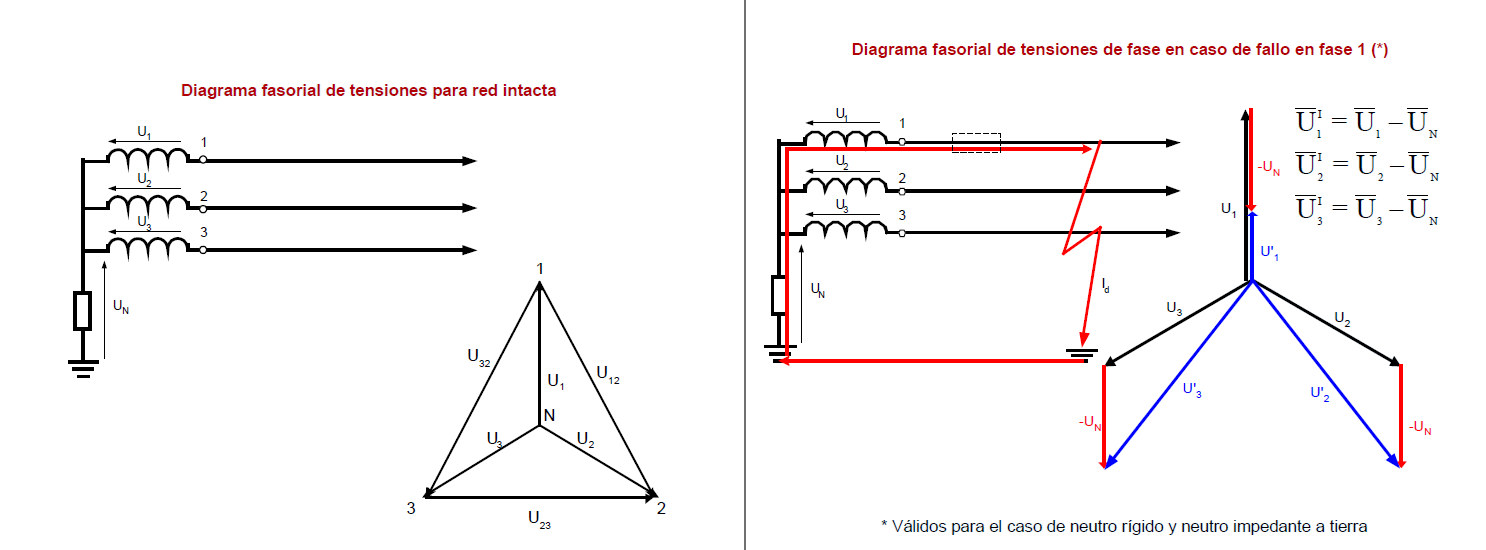
\includegraphics[width=1\linewidth]{Images/52}
	\label{fig:52}
\end{figure}
\begin{figure}[H]
	\centering
	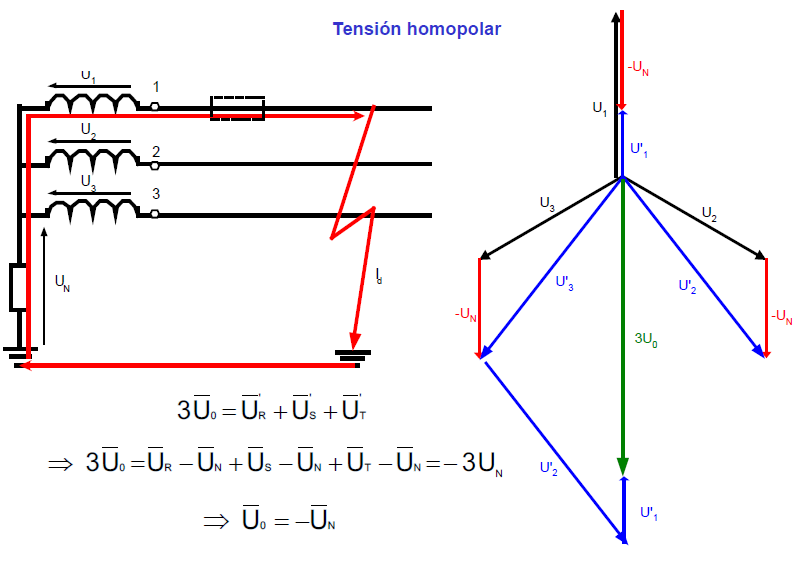
\includegraphics[width=0.7\linewidth]{Images/53}
	\label{fig:53}
\end{figure}
Cuando se dice que hay un fallo monofásico con un trafo monofásico, el trafo mide la suma de las 3 tensiones de fase, es decir, la homopolar.
\section{Neutro rígido a tierra}
Existe intensidad de defecto:
\begin{equation}
	I_d=\dfrac{-cU_1}{R_{PAT}+Z_T}\approx\dfrac{-cU_1}{Z_T}
\end{equation}
Se comporta como un neutro impedante de baja impedancia resistiva, la intensidad de defecto es de tipo inductivo. Se ajusta la protección $<U_0 - I_d> =\ang{180}$ inductiva.
\newline

Características
\begin{itemize}
	\item Fácil detección de las faltas a tierra
	\item	Inconveniente en AT: altas intensidades de defecto a tierra $\rightarrow$ $\uparrow$solicitación térmica, $\uparrow$corrientes por pantallas, $\uparrow$tensiones de paso y contacto
	\item	Ventaja: no aparecen sobretensiones en caso de derivación a tierra
	\item Aplicación:
	\begin{itemize}

	\item	Red de transporte (falta a tierra inductiva)
	\item	Red de distribución de BT (falta resistiva)
	\item	Red de distribución de MT	(tensiones MT bajas, en desuso )
\end{itemize}
\end{itemize}
\begin{figure}[H]
	\centering
	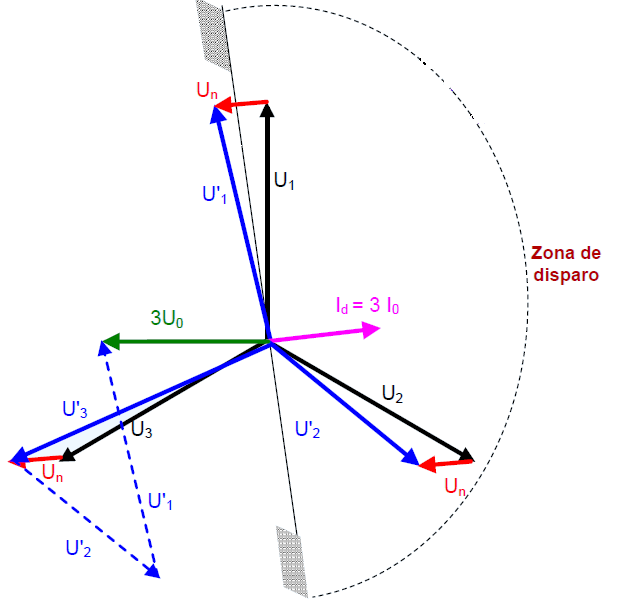
\includegraphics[width=0.43\linewidth]{Images/54}
	\label{fig:54}
\end{figure}


\section{Neutro impedante por resistencia}
Ventajas respecto a neutro rígido a tierra:
\begin{itemize}
	\item Limitación de la intensidad de defecto:
\begin{itemize}
	\item 	Menor solicitación térmica de faltas monofásicas
	\item Menores secciones de pantallas en cables MT
	\item Menores tensiones de paso y contacto en CT
\end{itemize}

	\item Posibilidad de selectividad cronométrica
\end{itemize}

Los esquemas de neutro pueden ser mediante:
\begin{itemize}
	\item Resistencia
	\item Reactancia
	\item Reactancia zig-zag (transformador de tierra)
\end{itemize}
\subsection{Soluciones para conseguir un tamaño viable para la resistencia}
\begin{figure}[H]
	\centering
	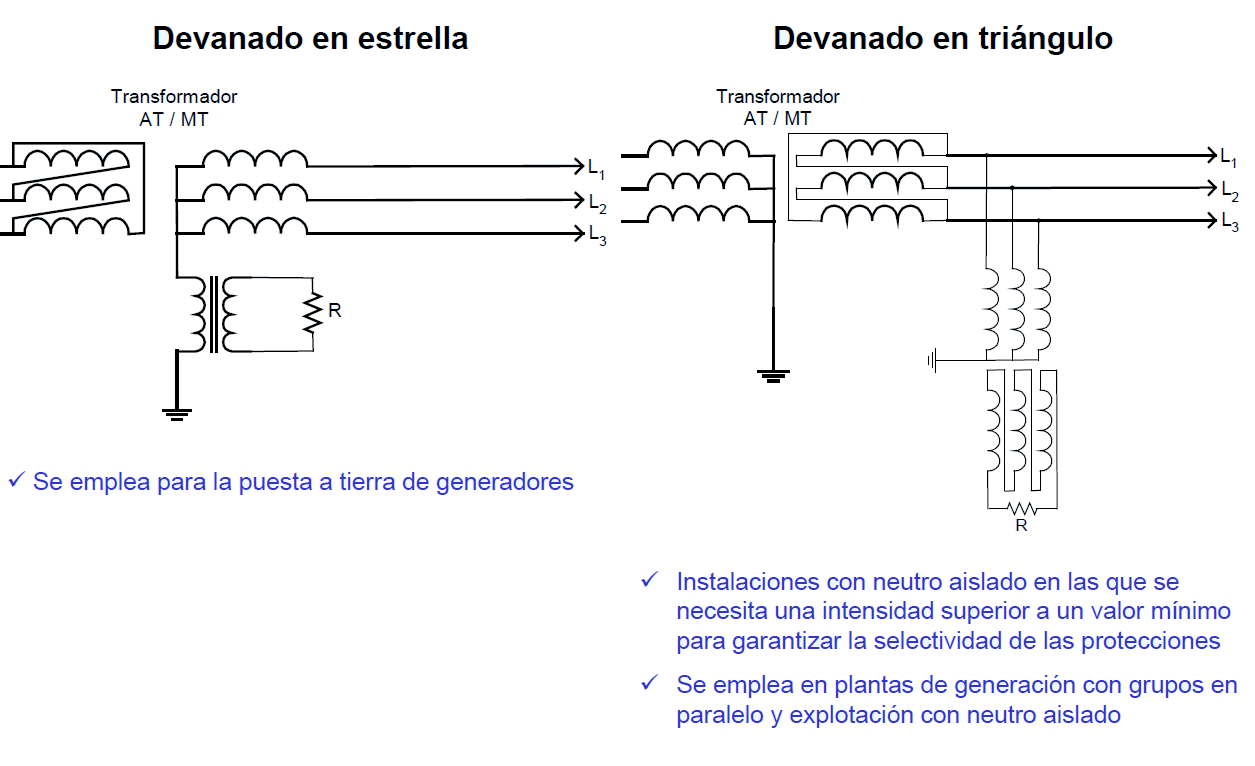
\includegraphics[width=0.65\linewidth]{Images/55}
	\label{fig:55}
\end{figure}
\subsection{Diagramas fasoriales}
La intensidad de defecto es de tipo resistivo-inductivo (mayormente resistivo).
\begin{equation}
	I_d=\dfrac{-cU_1}{R_N+Z_L+Z_T}\approx\dfrac{-cU_1}{R_N}
\end{equation}
\begin{figure}[H]
	\centering
	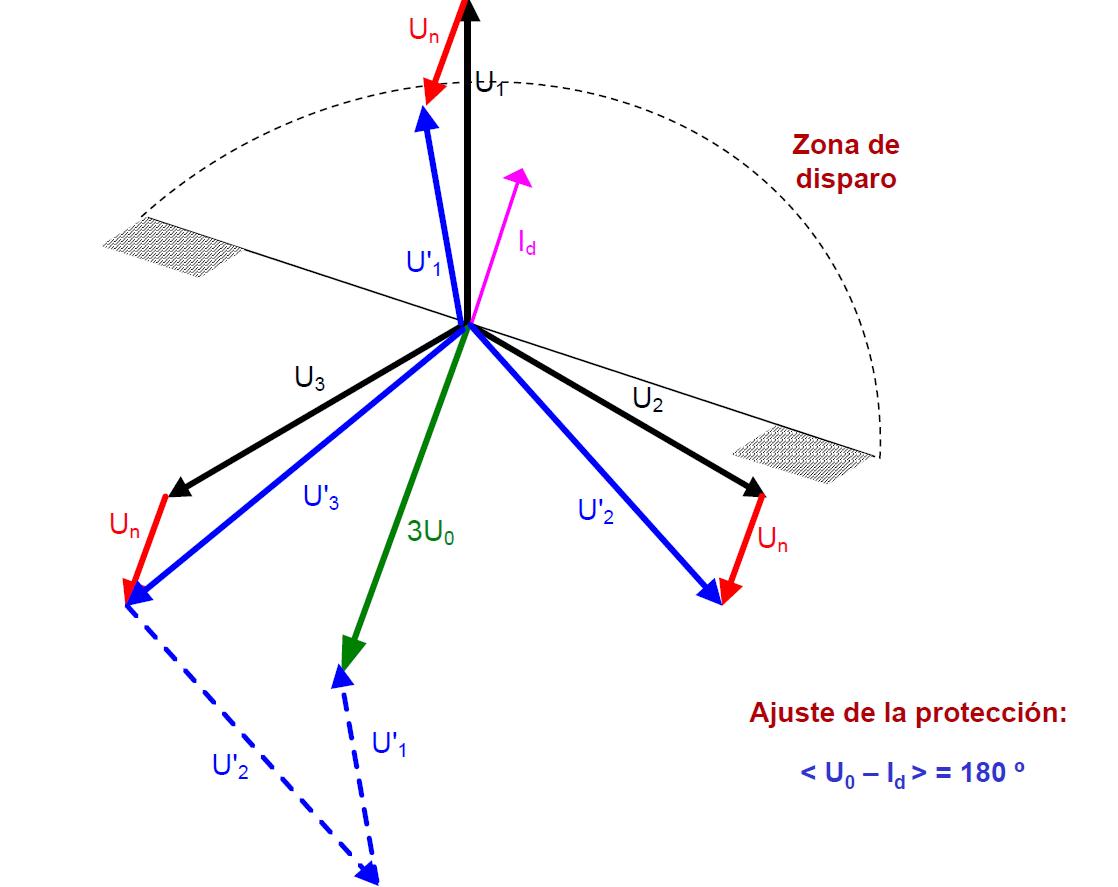
\includegraphics[width=0.43\linewidth]{Images/56}
	\label{fig:56}
\end{figure}

\section{Neutro impedante por reactancia}
Características:
\begin{itemize}
	\item Ventaja principal respecto a neutro impedante por resistencia: menor coste con intensidades de defecto altas y sin limitaciones
	\item Resonancia: es necesario comprobar que no se produce resonancia entre al reactancia del neutro y la capacidad a tierra de la red
	\item Diagrama fasorial similar al de neutro rígido a tierra
	\item Aplicación: redes de distribución de MT
\end{itemize}

Para poner el neutro mediante reactancia se conecta el centro de la estrella a tierra mediante una L.
\subsection{Neutro con impedancia Zig-Zag}
\begin{figure}[H]
	\centering
	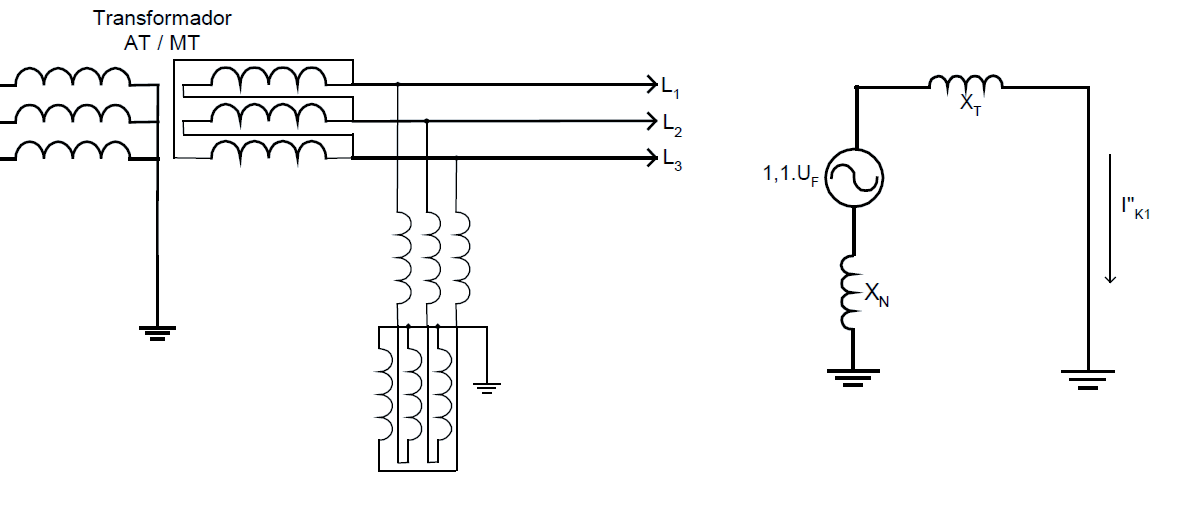
\includegraphics[width=0.7\linewidth]{Images/57}
	\label{fig:57}
\end{figure}
Características:
\begin{itemize}
	\item Solución para el caso de neutro no accesible
	\item Presenta sus mismas características
	\item Valores habituales de Id para redes de 20 kV de IBERDROLA: 500 A y 1000 A
	\item Debe comprobarse que no pueden aparecer fenómenos de resonancia entre la reactancia del neutro y la capacidad de la red
\end{itemize}
\newpage
\subsubsection{Neutro impedante por reactancia zig-zag y resistencia}
\begin{figure}[H]
	\centering
	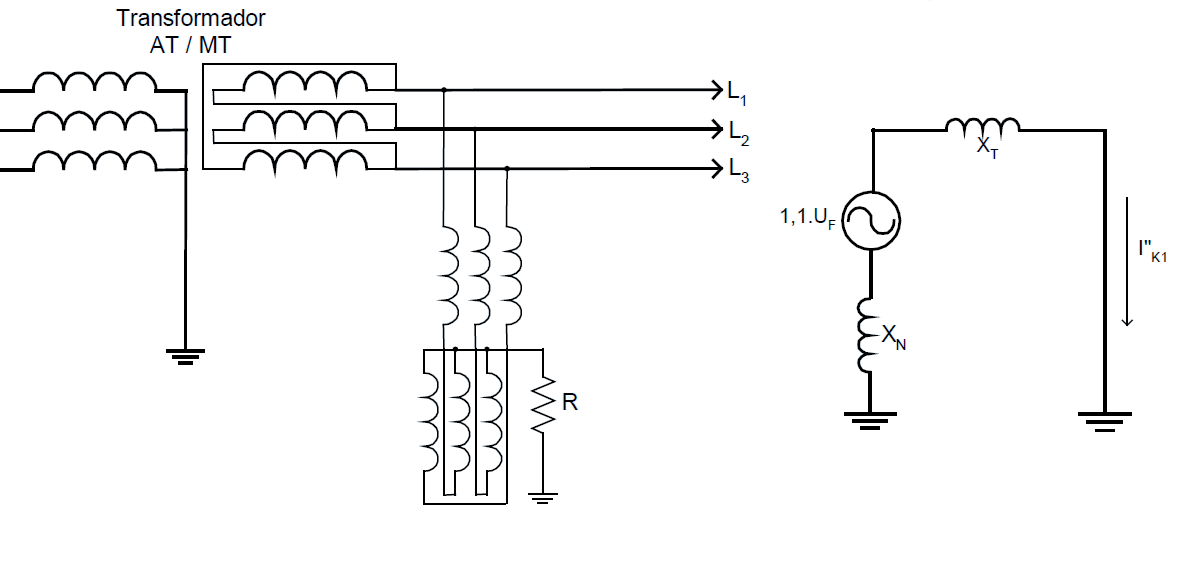
\includegraphics[width=0.7\linewidth]{Images/58}
	\label{fig:58}
\end{figure}
Características:
\begin{itemize}
	\item Disminución adicional de la corriente de falta a tierra sin un incremento de coste significativo
	\item Es el sistema de neutro impedante de mayor proyección futura
	\item Muy utilizado en plantas depuradoras donde los aportes de continua pueden ser importantes
\end{itemize}
\subsection{Esquema de red}
\begin{figure}[H]
	\centering
	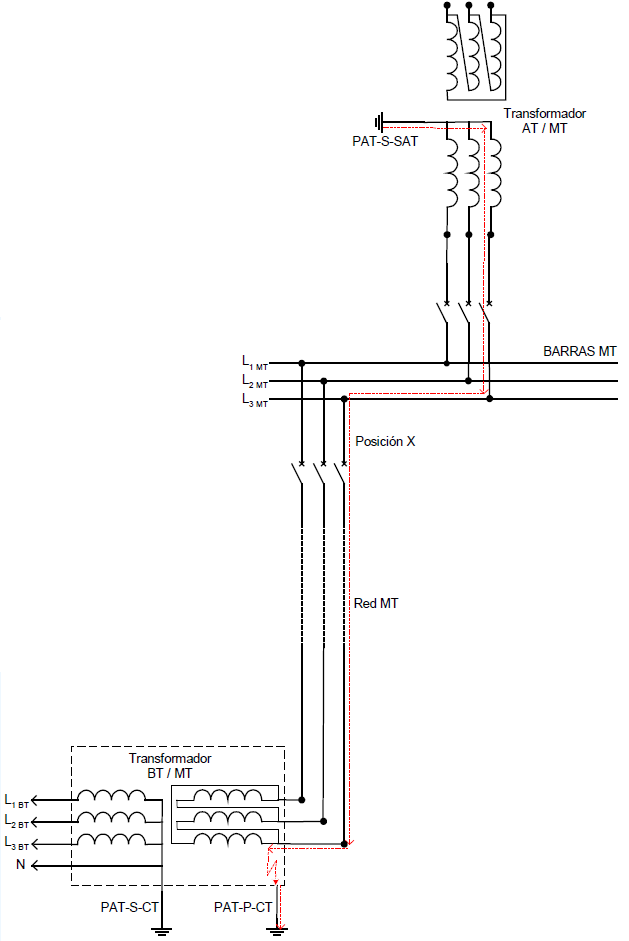
\includegraphics[width=0.4\linewidth]{Images/59}
	\label{fig:59}
\end{figure}

\section{Neutro aislado}
Características:
\begin{itemize}
	\item Ventaja principal: continuidad del servicio
	\item Sólo interrumpido por faltas polifásicas y monofásicas a tierra de larga duración
	\item Inconveniente: aparición de sobretensiones en caso de falta a tierra
	\item Es necesario conocer el valor mínimo de la capacidad a tierra, para que el ajuste de las protecciones sea suficientemente sensible
\end{itemize}
\begin{figure}[H]
	\centering
	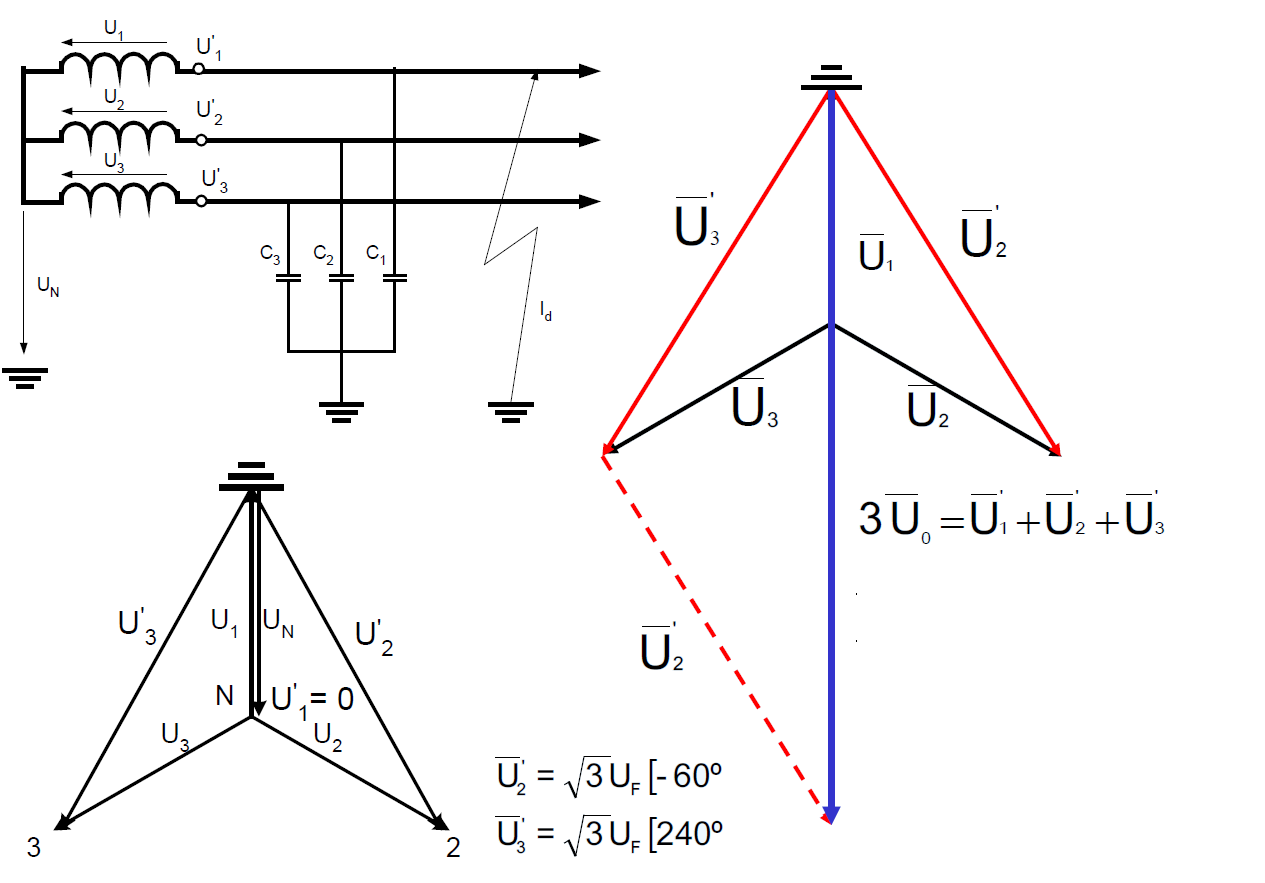
\includegraphics[width=0.7\linewidth]{Images/60}
	\label{fig:60}
\end{figure}
